\chapter{\heiti Software Usage}
\section{\heiti Open the software}
\hspace{-0.2cm}Open the folder `Integration', and double click file `ASG.py' to open the sequence editing software. The main interface is shown in Fig 4.1.
%进入我司为用户提供的Integration的文件夹,双击运行“ASG.py”文件,即可打开方波序列编辑软件。软件主界面(Pulse界面)如图4.1所示。
\begin{figure}[ht]
\centering
%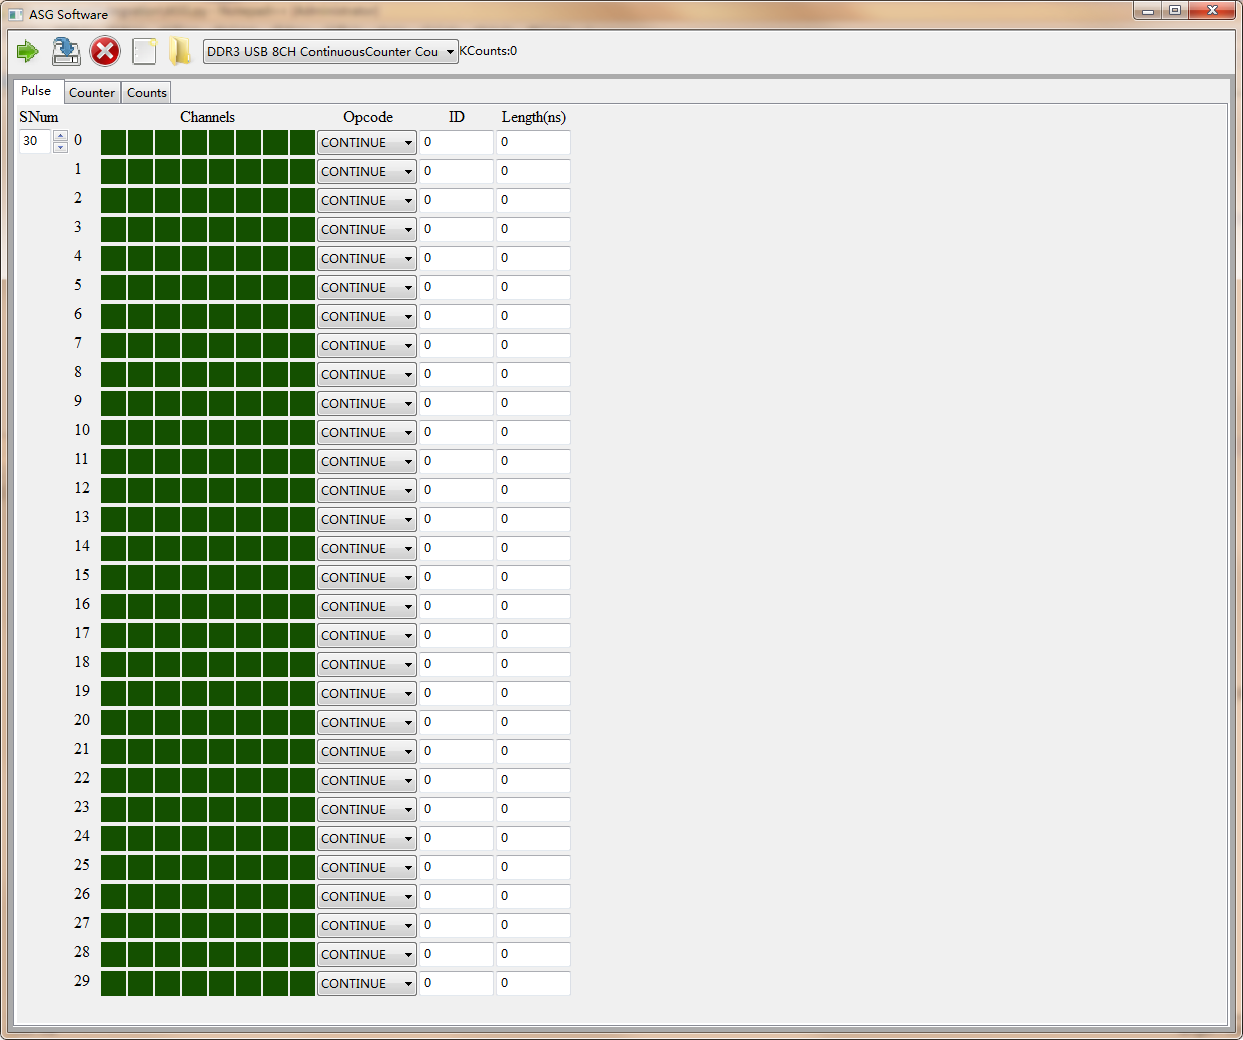
\includegraphics[width=11cm,height=9cm]{fig4_1}
%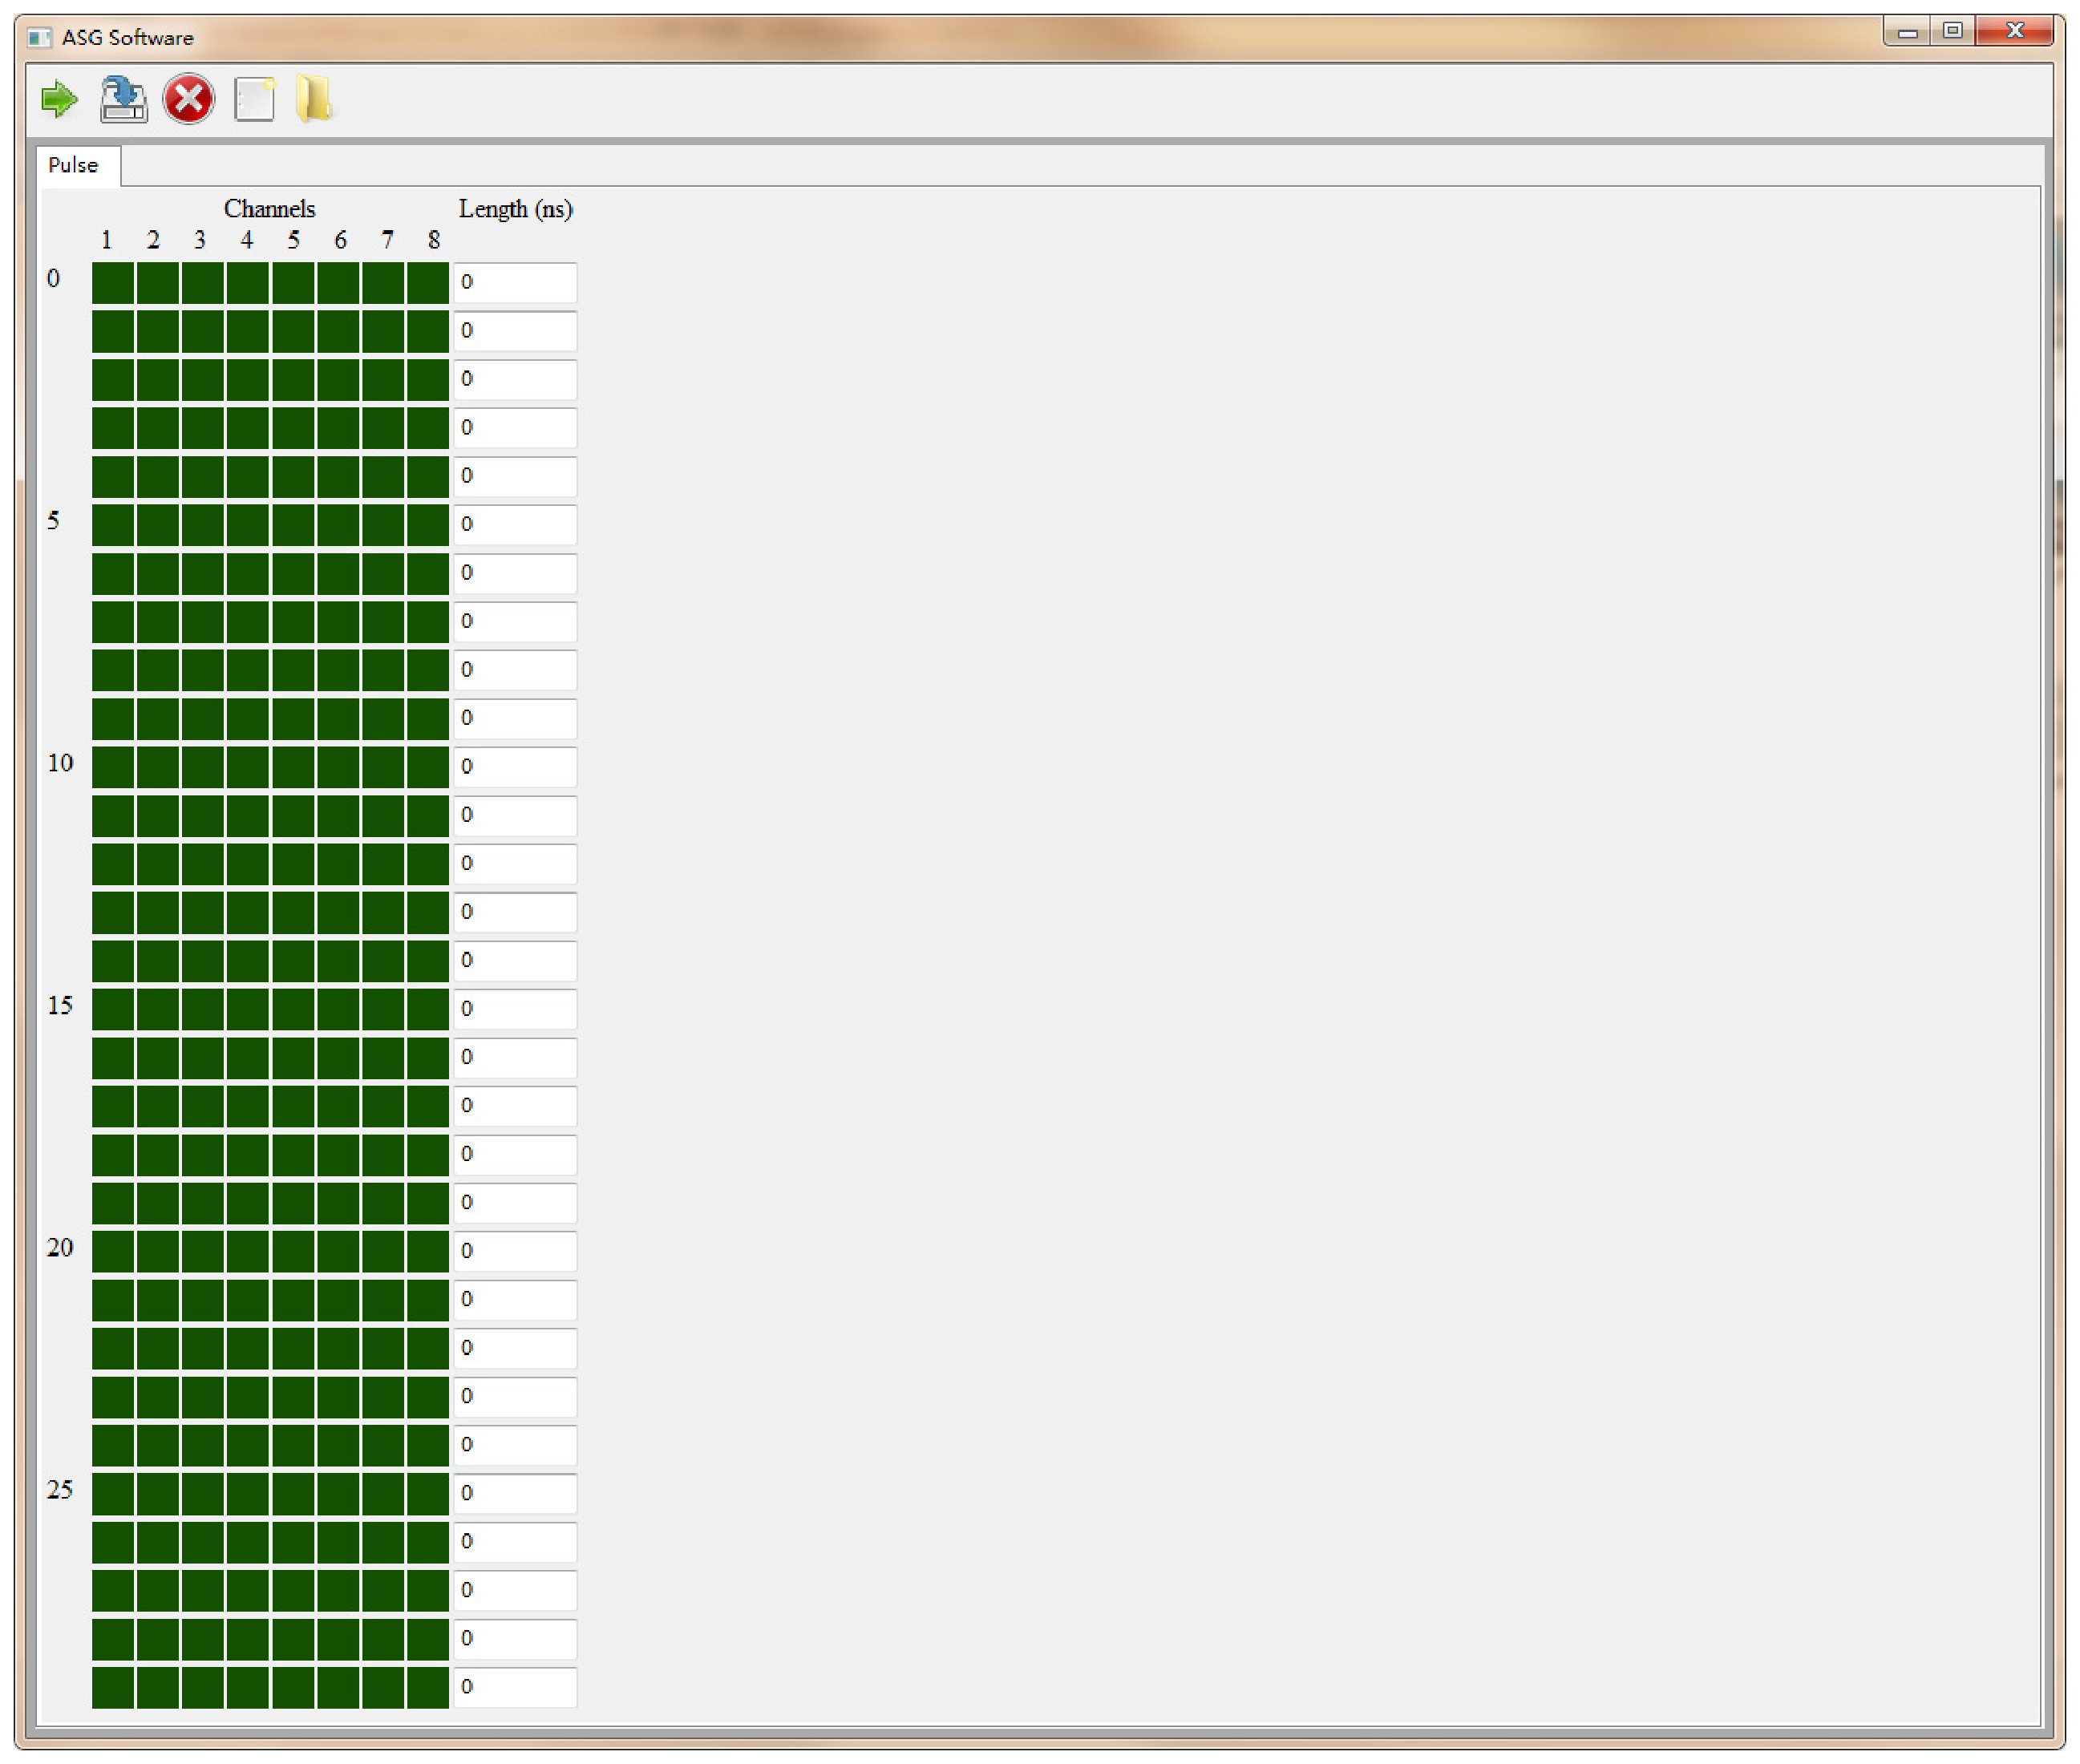
\includegraphics[width=12cm,height=9cm]{fig4_1_xyj}
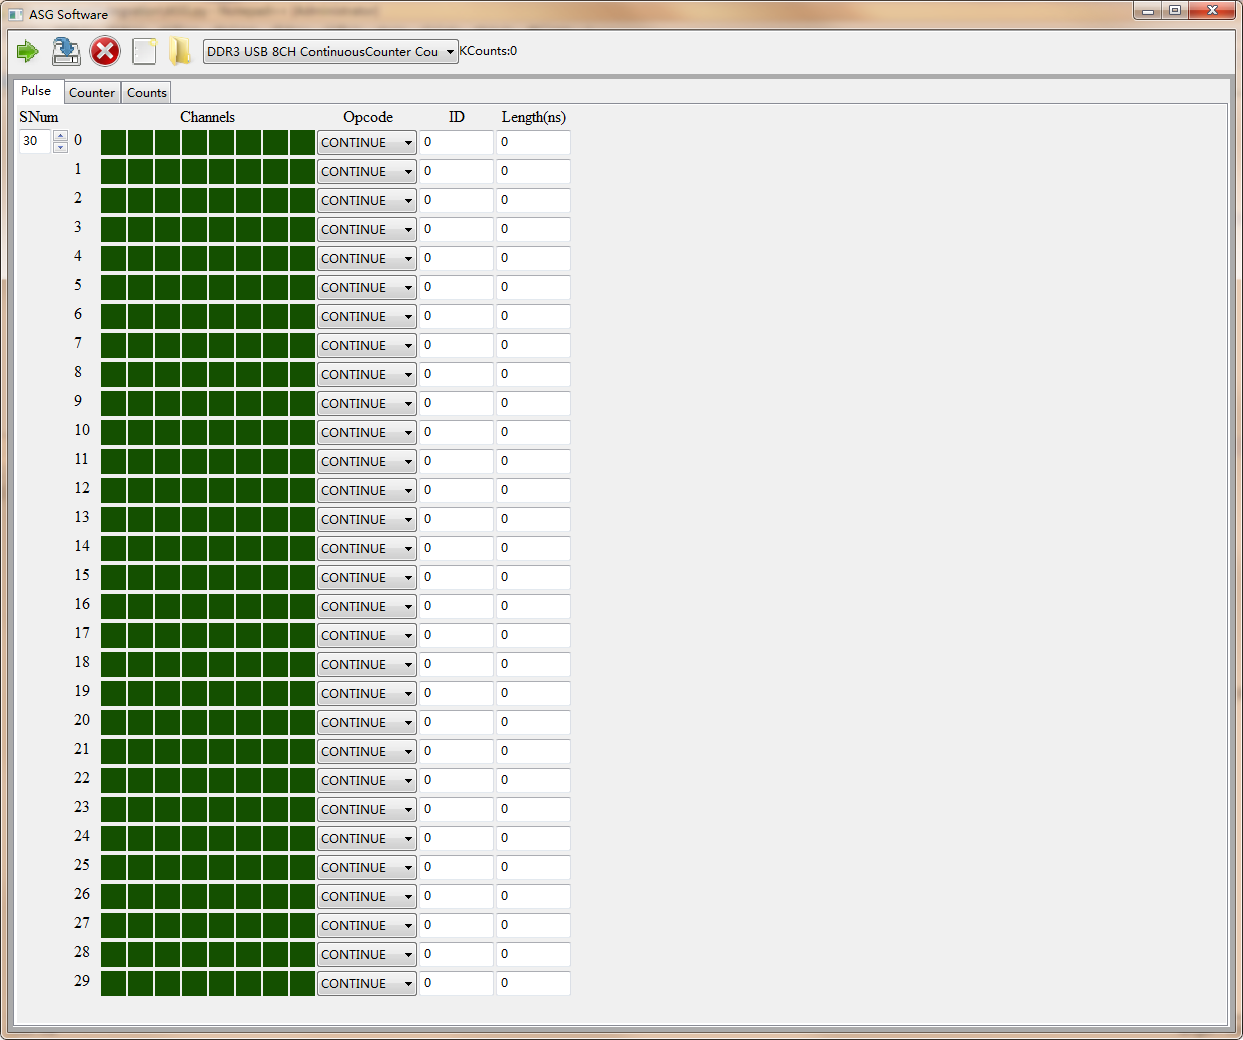
\includegraphics[height=9cm]{fig4_1}
\caption{\hspace{0.2cm}Main interface of the software}
\end{figure}

\hspace{-0.2cm}There are five buttons in the toolbar of the software: `Start', `Download', `Stop', `Loadfile' and `Save'. The 8 green boxes each row in the interface represent the condition of  8 output channels. When the box is lit up, the channel output positive pulse, if  not, the channel output negative pulse, the length of time is depend on the number in the textbox, and the unit is nanosecond.
%在软件主界面工具栏中,从左往右5个按钮依次为:“开始播放按钮”、“下载方波数据按钮”、“停止播放按钮”、“存储当前方波序列按钮”、“载入存储方波序列按钮”。界面中间的每行8个绿色方框,从左往右依次代表OUT 1 至OUT 8 的8 个方波输出通道在一段时间内的输出状态(时间长度由右侧的“Length” 文本框内输入的数值决定,单位为纳秒)。当绿色被点亮时,该通道在此段时间内的输出为高电平;若绿色未被点亮,则该通道在此段时间内的输出为低电平。

\section{\heiti Define arbitrary sequence}
\hspace{-0.2cm}User can define arbitrary sequences depend on the condition of the boxes and the length of time. In Fig 4.2, `CH - 1' to `CH - 4' represent 4 output channels, if users want to define sequences like Fig 4.2, they can define the sequences as Fig 4.3.
%用户可根据每行绿色方框的不同状态及“Length”的长度来定义任意的方波序列。如图4.2,左侧“CH - 1”至“CH - 4” 代表4个方波输出通道,若用户想要生成如图4.2所示的方波序列,可如图4.3在软件界面中定义该方波序列。

\newpage
\vspace{0.6cm}
\begin{figure}[H]
\centering
%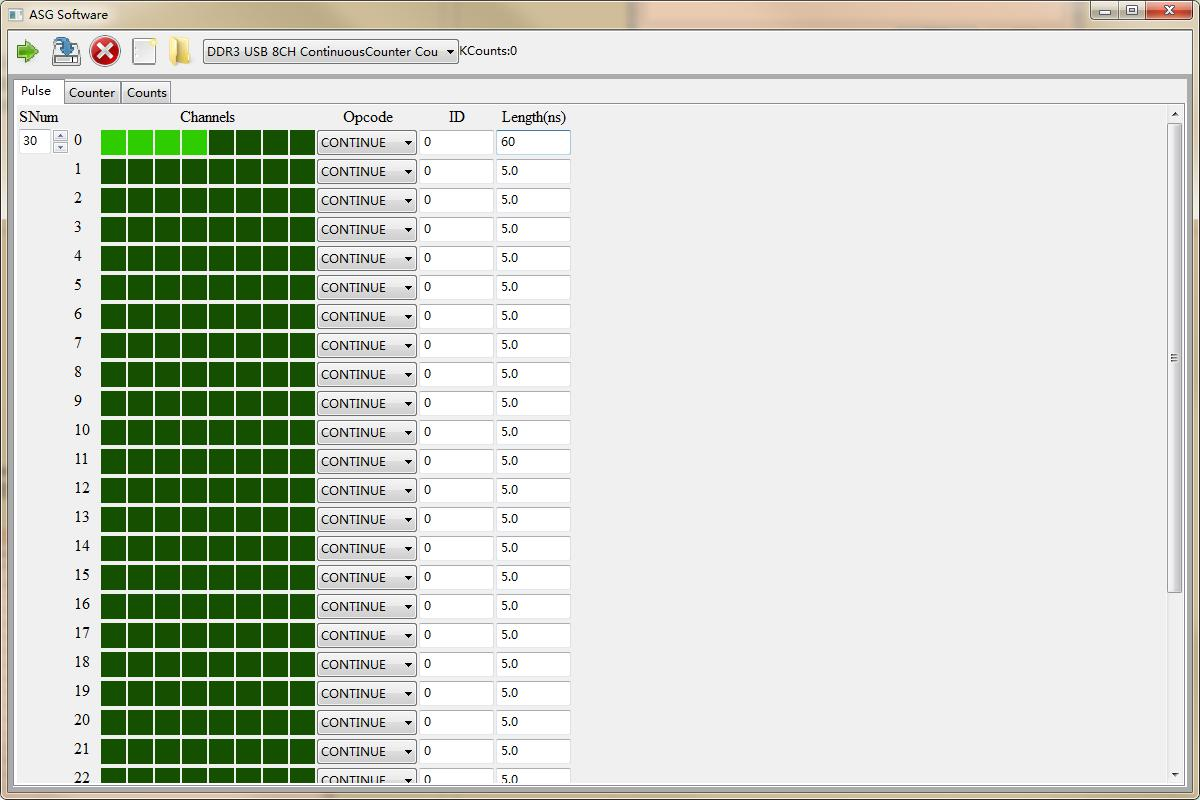
\includegraphics[width=11cm,height=9cm]{fig4_2}
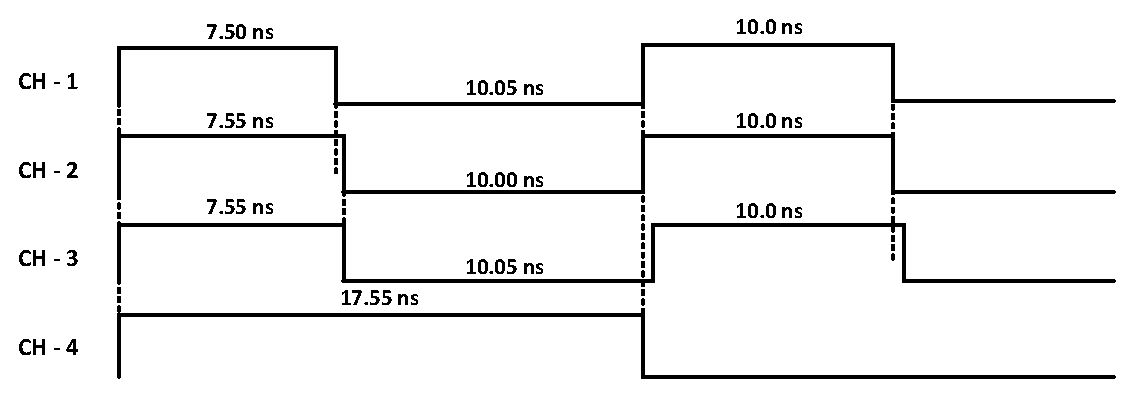
\includegraphics[height=5cm,width=14cm]{fig4_2_shixutu}
\caption{\hspace{0.2cm}Customize timing diagram of pulse signal}
\end{figure}

\vspace{1cm}
\begin{figure}[H]
\centering
%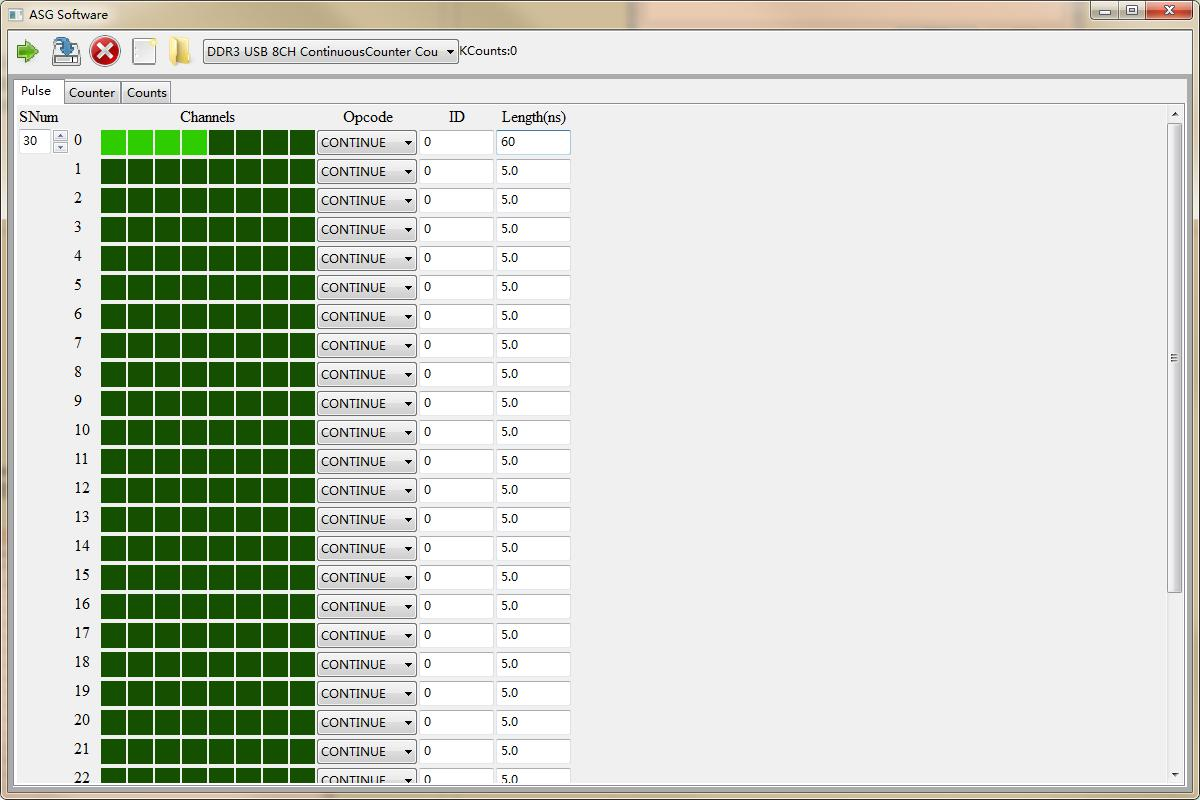
\includegraphics[width=11cm,height=9cm]{fig4_2}
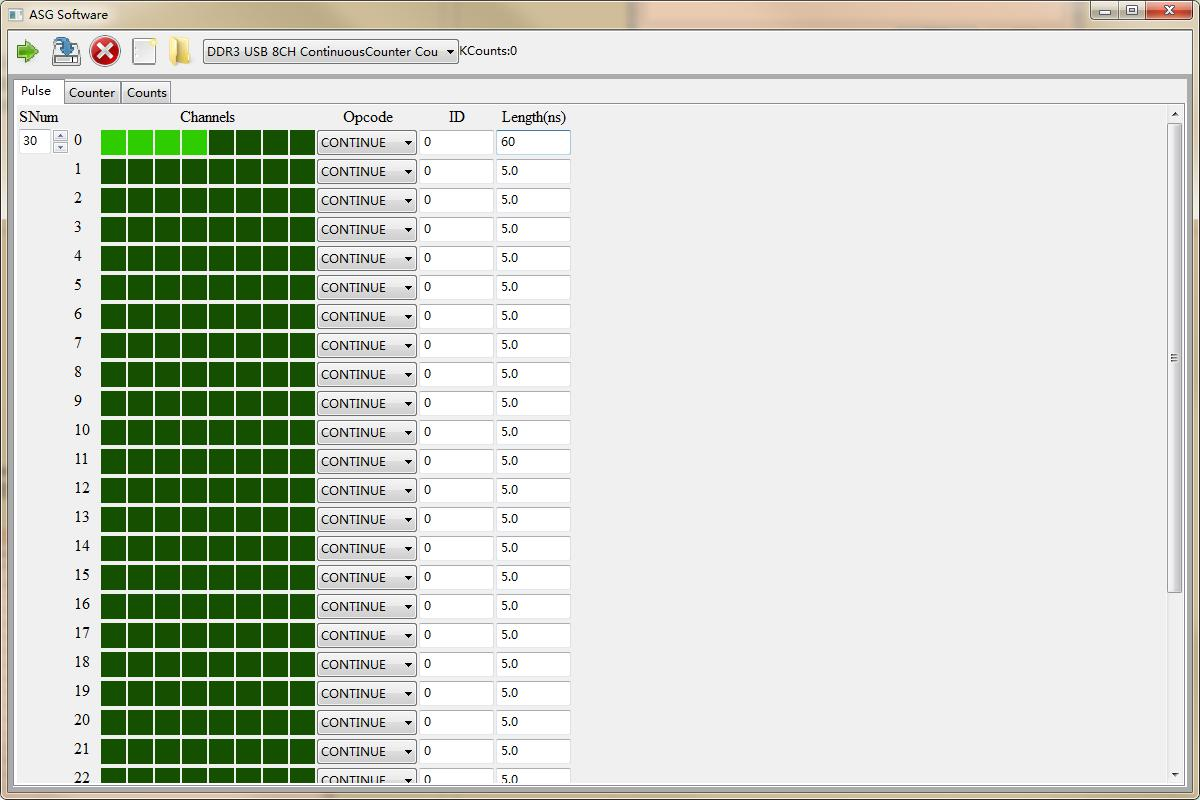
\includegraphics[height=9cm]{fig4_2}
\caption{\hspace{0.2cm}Use software to define the sequence}
\end{figure}
\vspace{0.1cm}
\hspace{-0.2cm}As Fig 4.3, users can use the software to define the sequences as Fig 4.2. Only 4 channels are used in Fig 4.3, if users need more output channels, please define the sequences the same way in other channels.
%如图4.3使用方波编辑软件定义图4.2中的方波序列,这里只使用了4个方波输出通道,若用户需要同时使用更多的方波输出通道,可用同样的方法在其他通道定义任意方波序列。

\section{\heiti Start playing the sequence}
\hspace{-0.2cm}Users can click `Download' button 
\includegraphics[height=0.6cm]{download} to download the data of the sequence into the hardware. Then click `Start' buttton 
\includegraphics[height=0.6cm]{start} to play the sequence. For example, if you define the sequence as Fig 4.2, you can see the waveform as Fig 4.4 on the oscilloscope.
%用户点击“Download”按钮
\includegraphics[height=0.7cm]{download},可将自定义的方波序列数据下载到硬件中。点击“Start”按钮
\includegraphics[height=0.7cm]{start},可使仪器各输出通道开始播放用户自定义的方波序列,在点击“Start” 按钮之前必须先将方波序列数据下载到硬件中。将输出通道用同轴线连接至示波器上可以看到仪器输出的方波波形。如用户定义图4.2所示方波序列,在示波器上可以看到如图4.4 所示的方波序列。

%\vspace{1cm}
\begin{figure}[htbp]
\centering
%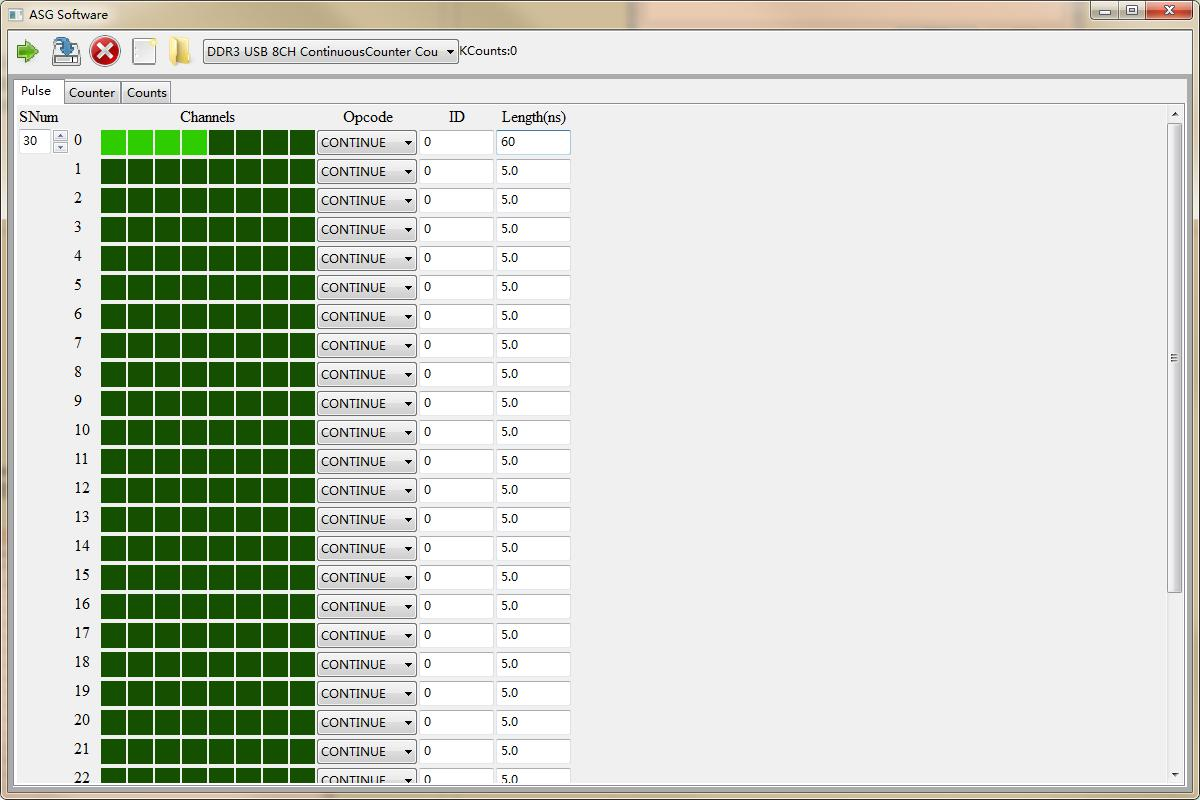
\includegraphics[width=11cm,height=9cm]{fig4_2}
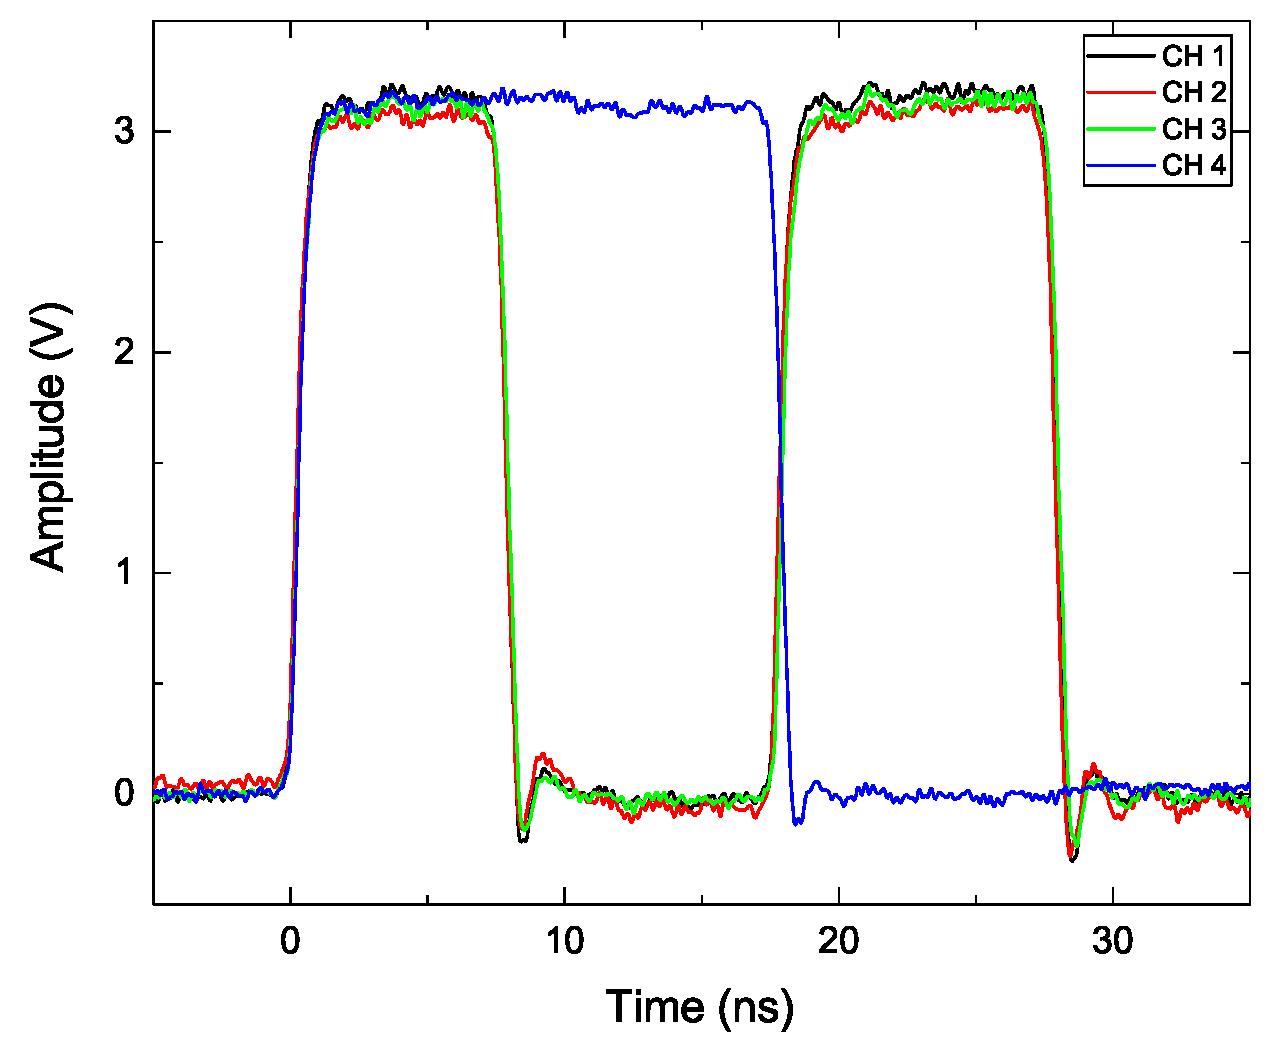
\includegraphics[height=9cm]{yangheng_shiboqi}
\caption{\hspace{0.2cm}The product output pulse sequence diagram}
\end{figure}

\section{\heiti Stop playing the sequence}
\hspace{-0.2cm}When the instrument is playing the sequence, users can click `Stop' button 
\includegraphics[height=0.6cm]{stop} to stop it.
%当仪器正在播放方波序列时,可以通过点击“Stop”按钮
\includegraphics[height=0.7cm]{stop}使仪器停止播放方波序列。

\section{\heiti Notices in defining the sequence}
%\section{\heiti 定义方波序列注意事项}

\vspace{0.4cm}
\noindent \textbf{(1)}. The minimum width of single pulse is 7.5 ns. As Fig 4.5, if users define the length

\hspace{0cm}of single pulse is shorter than 7.5 ns, the warning dialog will pop up.
%\noindent \textbf{(1)}. 每个通道的方波序列中单个方波脉冲的高低电平时间必须在7.5 ns至2.6 s以内。如图4.5,当用户定义的方波序列中单个脉冲宽度小于7.5 ns 时,软件会弹出提示对话框让用户检查自定义的方波序列是否符合要求。

\vspace{0.2cm}
\begin{figure}[H]
\centering
%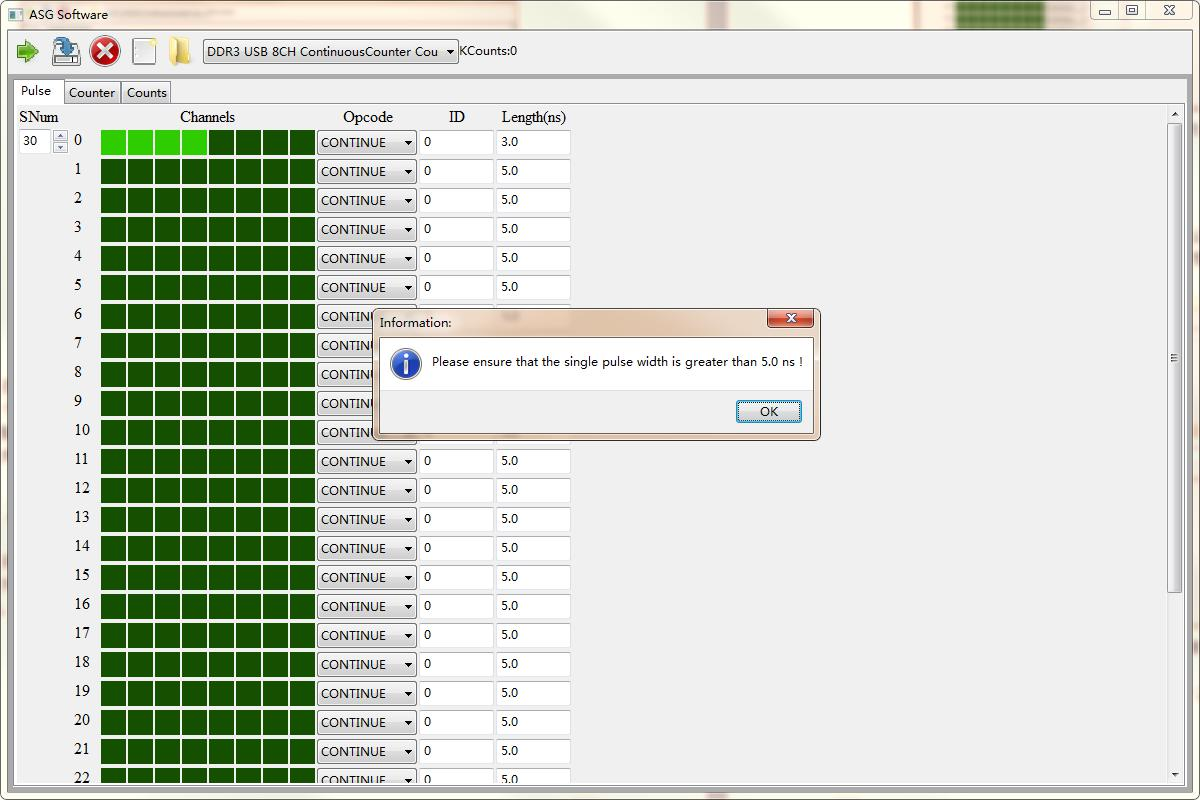
\includegraphics[width=11cm,height=9cm]{fig4_3}
%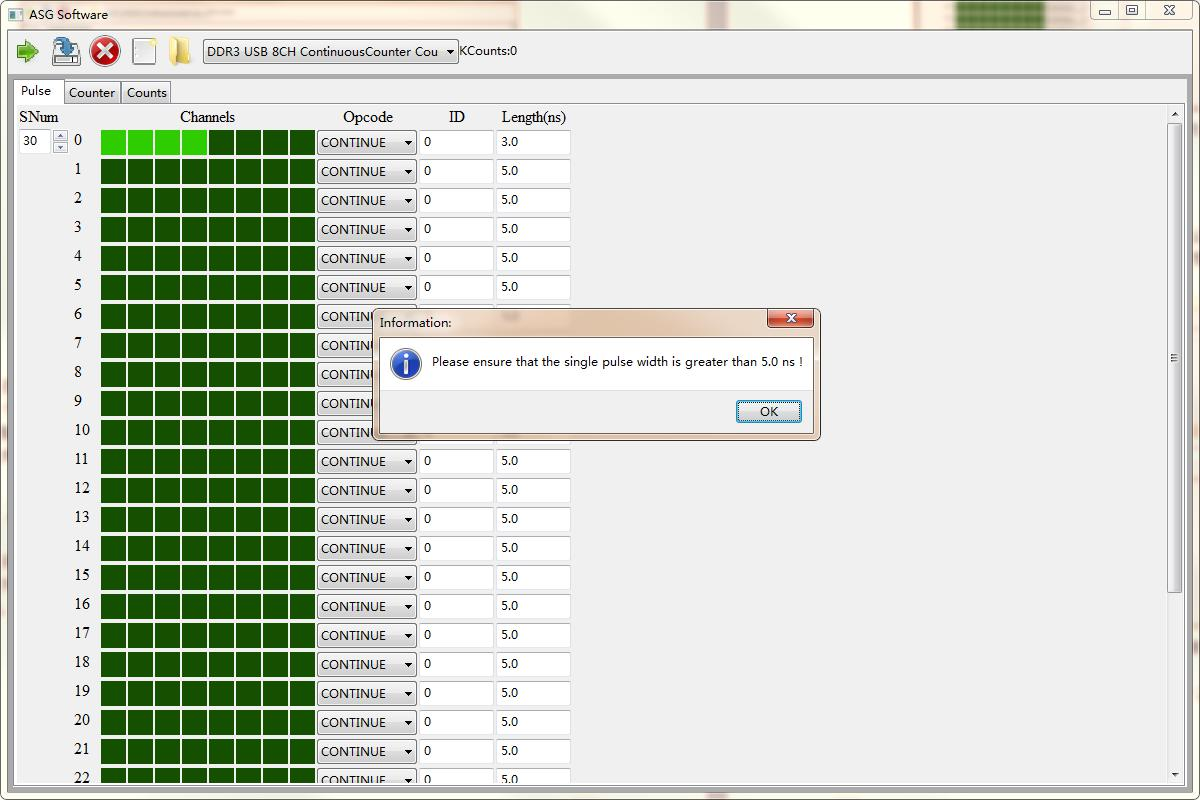
\includegraphics[height=9cm]{fig4_3}
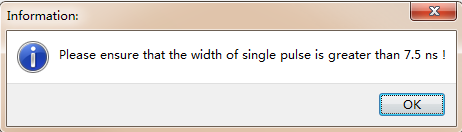
\includegraphics[height=3cm]{fig4_5_yh}
\caption{\hspace{0.2cm}The length of single pulse must be greater than 7.5 ns}
\end{figure}

%\newpage
\vspace{0.4cm}
\noindent \textbf{(2)}. The maximum width of single pulse is 2.6 s. As Fig 4.6, if users define the length 

\hspace{0cm}of single pulse is greater than 2.6 s, the warning dialog will pop up.

%\noindent \textbf{(2)}.  如图4.6,当用户定义的方波序列中单个脉冲宽度大于2.6 s时,软件会弹出提示对话框。

\vspace{0.2cm}
\begin{figure}[ht]
\centering
%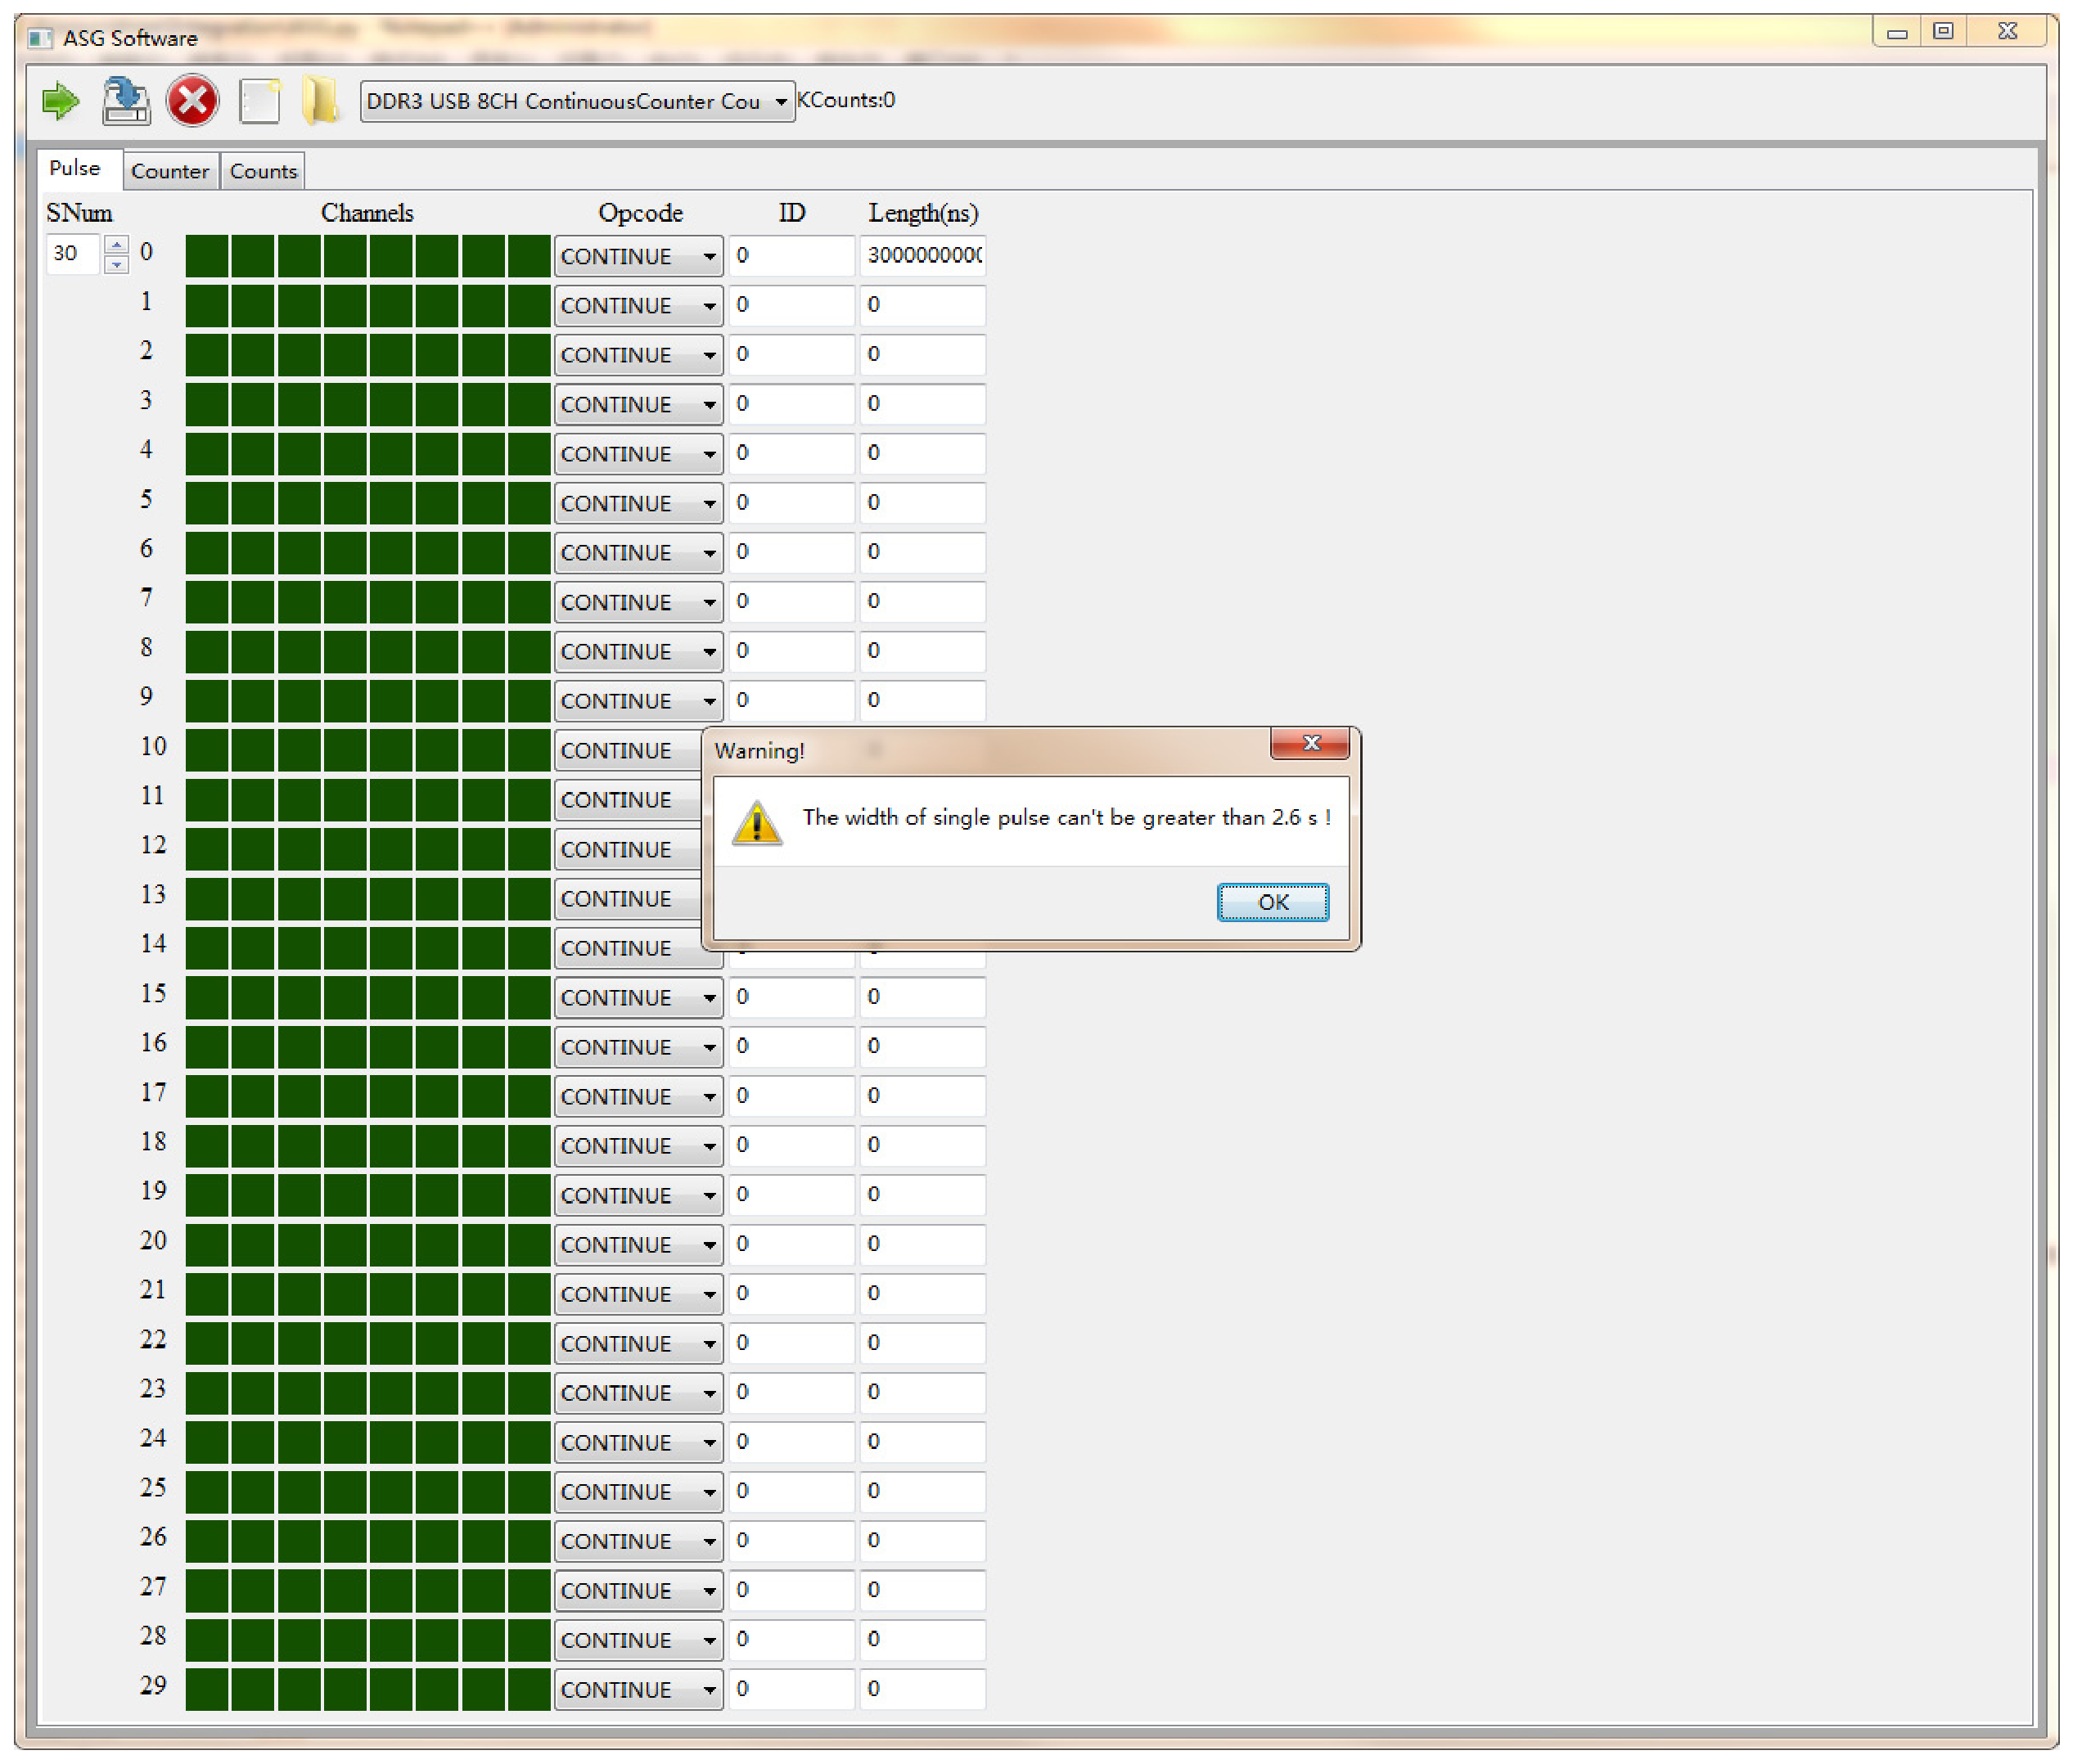
\includegraphics[width=11cm,height=9cm]{fig4_4}
%\includegraphics[height=9cm]{fig4_4yh}
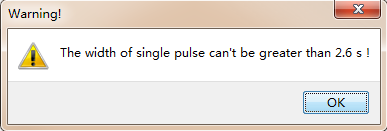
\includegraphics[height=3cm]{fig4_6_yh}
\caption{\hspace{0.2cm}The length of single pulse must be shorter than 2.6 s}
\end{figure}

\vspace{0.4cm}
\noindent \textbf{(3)}. As Fig 4.7, if users define the length of single pulse is not integral multiple of

\hspace{0cm}0.05 ns, the warning dialog will pop up.
%\noindent \textbf{(3)}. 用户定义的每个方波序列的宽度必须是0.05 ns的整数倍。如图4.7,当用户定义的方波序列中存在单个方波脉冲宽度非0.05 ns整数倍时,软件会弹出提示对话框。

\vspace{0.2cm}
\begin{figure}[H]
\centering
%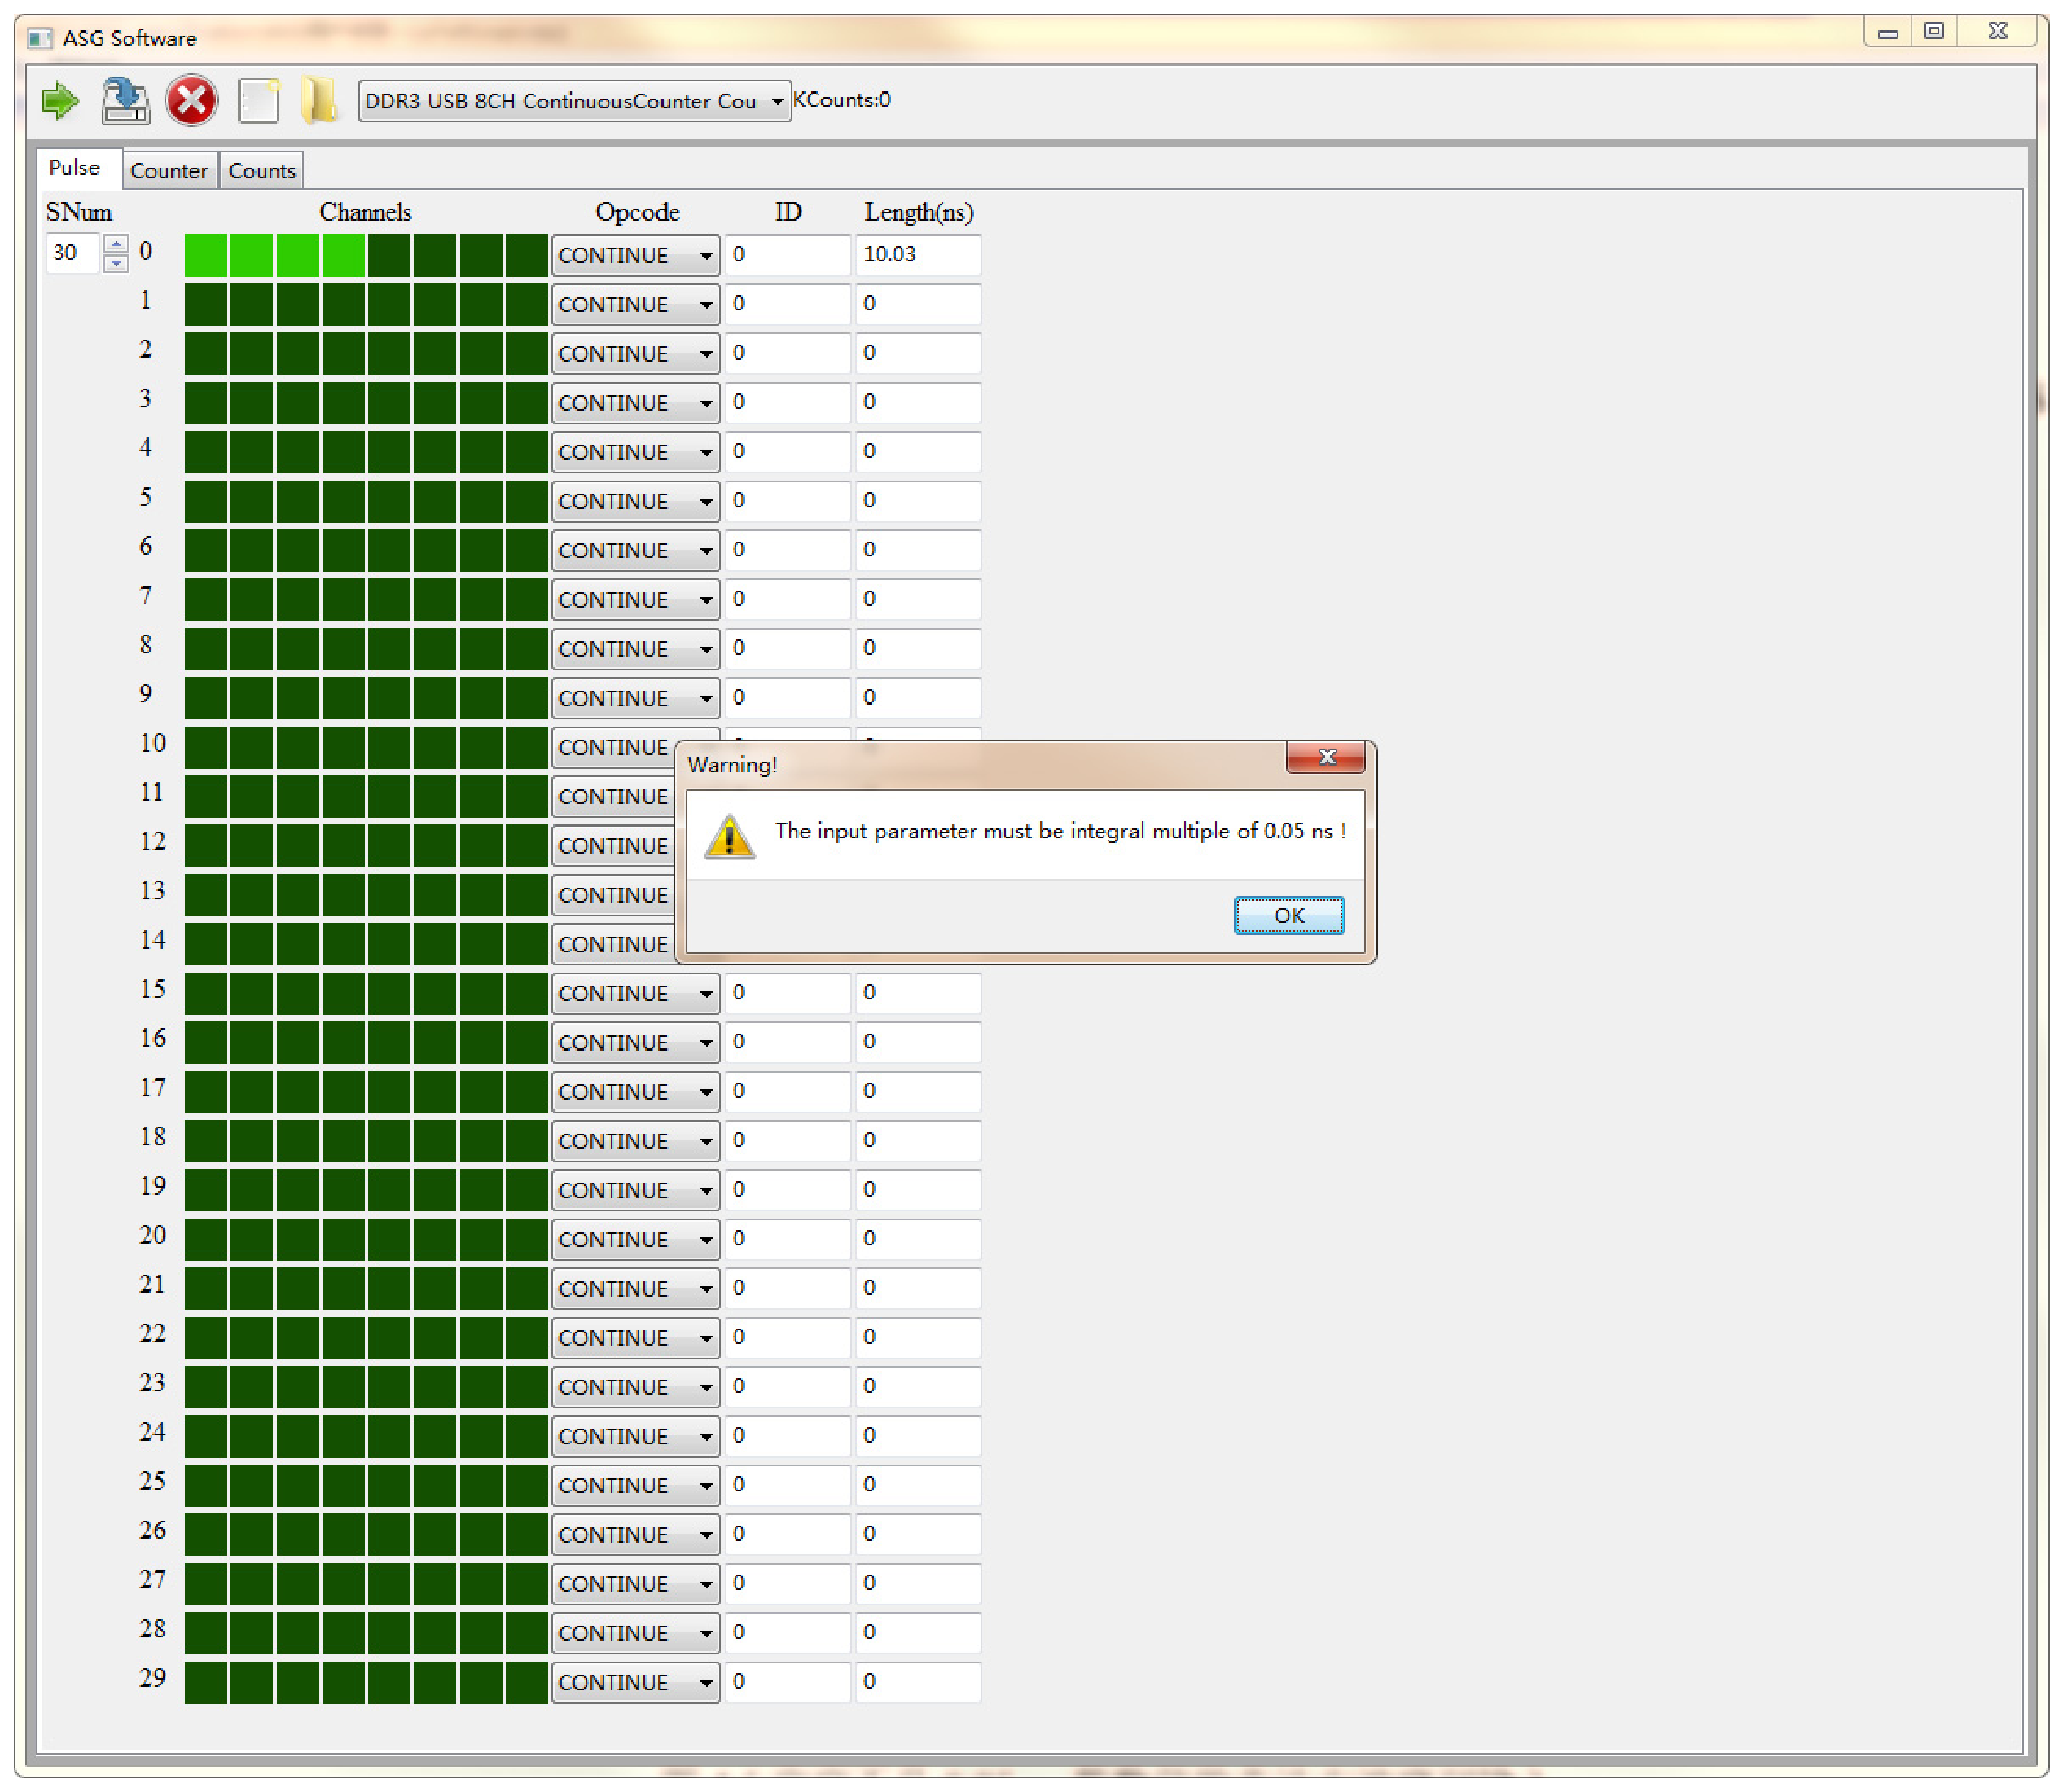
\includegraphics[width=11cm,height=9cm]{fig4_5}
%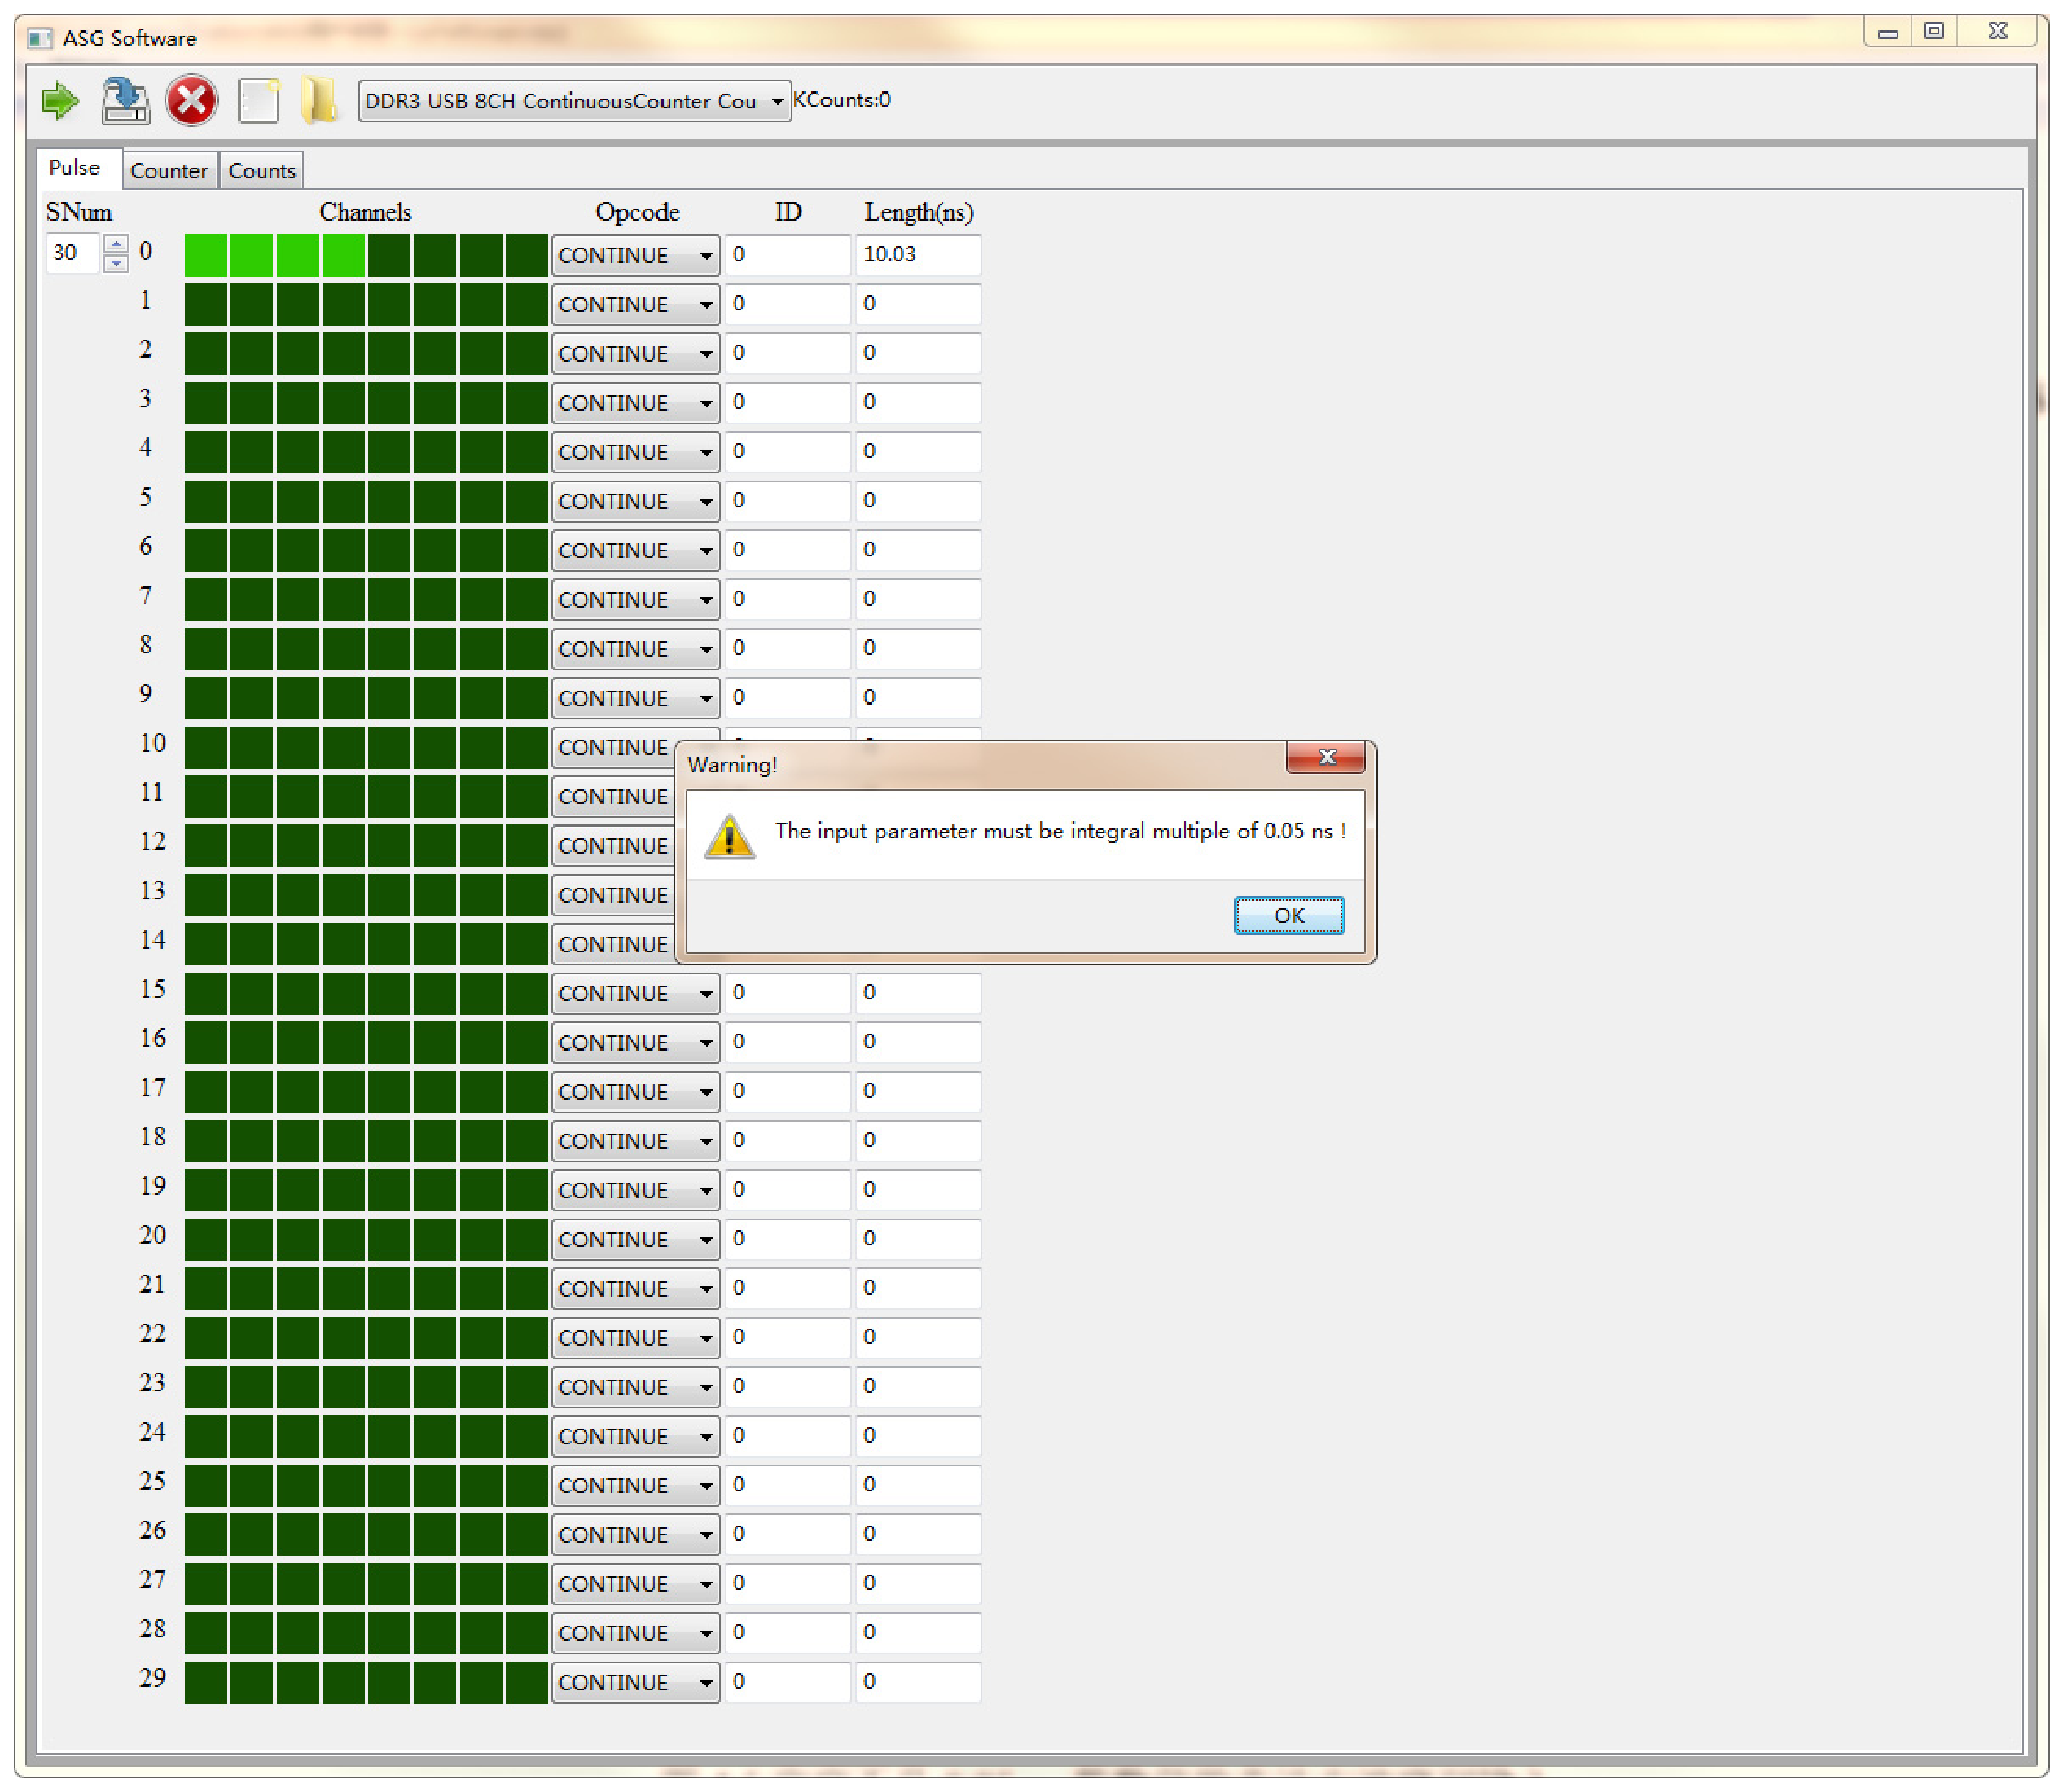
\includegraphics[height=9cm]{fig4_5}
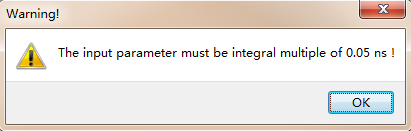
\includegraphics[height=3cm]{fig4_7_yh}
\caption{\hspace{0.2cm}The length of single pulse must be integral multiple of 0.05 ns}
\end{figure}

%\newpage
%\section{\heiti 开始播放方波序列}
%用户点击“Download”按钮
%
\includegraphics{download},可将自定义方波序列数据下载到硬件中。点击“Start”按钮{ }{ }
\includegraphics[height=0.7cm]{start},可使仪器各输出通道开始同步播放用户自定义的方波序列,在点击“Start” 按钮之前必须先将方波序列数据下载到硬件中。将输出通道用同轴线连接至示波器上可以看到仪器输出的方波波形。
%
%\section{\heiti 停止播放方波序列}
%当仪器正在播放方波序列时,可以通过点击“Stop”按钮{ }{ }
\includegraphics[height=0.7cm]{stop}使仪器停止播放方波序列。





